\documentclass[12pt]{article}
\usepackage{setspace, graphicx, fullpage, amssymb, amsmath, epsfig, natbib, array, multirow, hyperref}
\usepackage{amsfonts, bm} 
\usepackage{dcolumn}
\usepackage{subfigure, float} 
\usepackage[margin=1in]{geometry} 
\usepackage{verbatim}
\usepackage{url}
\usepackage{enumerate}
\usepackage{morefloats}
\usepackage{caption}
\newcolumntype{d}[1]{D{.}{.}{#1}} 

\newcommand\fnote[1]{\captionsetup{font=small}\caption*{#1}}

\begin{document}
	\title{Who Heeds the Call in the U.S. Senate? Reelection and Member Responsiveness to the Party}
	
	\author{Ethan Hershberger\\Ohio State University \and William Minozzi\\Ohio State University \and Craig Volden\\University of Virginia \thanks{We would like to thank Andrew Podob for reviewing a draft of this paper.}}
	
	\date{\today}

\maketitle

\thispagestyle{empty}

\begin{abstract}
	\singlespacing
	\noindent
	In this paper, we replicate the findings of \cite{Minozzi:2013} with some modifications of their methodology. We show that their hypotheses regarding party unity coming through the party working to unite more extreme (rather than more moderate) members holds not only in the House, but also the Senate. Further, we show the usefulness of separating votes in this way by considering changes in member behavior when they are up for reelection.
\end{abstract}

\pagebreak
\setcounter{page}{1}

\doublespacing


\subsection*{Introduction}

\cite{Minozzi:2013} developed the notion of the `party call' vote as one in which the party is a factor in vote choice when accounting for ideology. Party call votes were hypothesized by the authors to produce party unity through calling on all members to support the party's position, rather than just pressuring moderates. These allow parties to display unity and establish their brand. While party calls can happen on numerous types of votes and issues, member response to the party call is hypothesized to be explained by member ideological placement. Their central hypothesis (the `responsive extremists hypothesis') was that the most extreme members of a party would be the most likely to vote with their copartisans on a party call vote. Minozzi \& Volden tested this in Congresses 93-109 in the House of Representatives. This study intends to replicate their findings with extensions into Congresses 110-112 as well as the Senate.

Additionally, we want to consider other areas which party calls may be helpful in explaining member behavior. We view the party call as a valuable tool in explaining member behavior in relation to their party. By defining areas in vote choice which the party is present beyond ideology, one can view separate aspects of their roles. The high correlation between party and ideology often can lead to misattributions in research \cite{Krehbiel:1993, Lee:2009}. It is now helpful to consider what we know and expect about party and ideology during our period of analysis.

Presently, parties are held to be increasingly polarized in both chambers of Congress \cite{Lee:2009, Lee:2016, Theriault:2013, Smith:2014}. Increased ideological extremism could potentially give members benefits for bucking the party, but a recognition of increasing partisanship and party brand management in recent Congresses \cite{Lee:2009, Lee:2016} leads us to expect party calls to instead  be more present in these periods. We additionally expect that the responsive extremists hypothesis will explain member behavior in both chambers on party call votes.

In extending results to consider reelection in the Senate, we recognize that it has been shown to influence member response to their party \cite{Levitt:1996}. This is unsurprising, since members' primary goal is reelection \cite{Mayhew:1974} and members are electorally punished for being out of line with their district or too in line with their party \cite{Canes-Wrone:2002, Carson:2010}. Party call votes would give them a clear opportunity to differentiate themselves from the party in the eyes of their constituents. Thus, we should expect Senators to be less responsive to party calls when they are up for reelection.

We find, as hypothesized, that party calls are present in the Senate and that they are on the rise in both chambers in Congresses 93-112. Further, we are able to show that members are less responsive to party calls when they are up for reelection at the end of a Congress. We take this as strong evidence that the party call vote is explaining partisan (and member) brand management in the legislature. In the next section we show the results of our replication with the section following it dedicated to additional tests concerning reelection before concluding the paper.

\subsection*{Replication}

In this section we detail the results of our replication models. To sort roll call votes as `party calls' and `party free votes' we used a modified version of the algorithm described in Minozzi \& Volden (2013).\footnote{A thorough overview of the algorithm highlighting changes we've made to it is found in an appendix} As in theirs, sorting was based on whether vote choice was significantly predicted by party status when controlling for ideology. For each iteration, member ideological positions were calculated on the party free votes from the previous iteration. We used this measure (with sign reversed for Democrats) to obtain member ideological extremism. 

We find, as expected, that party calls are present in both the House and Senate. Additionally, we find that in both chambers their incidence has been on an upward trend during our period of analysis (1973 - 2013), which we show in Figure 1. 


\begin{figure}[H]
	\centering
	\caption{Party Calls as a Percentage of Votes, Congresses 93-112}
	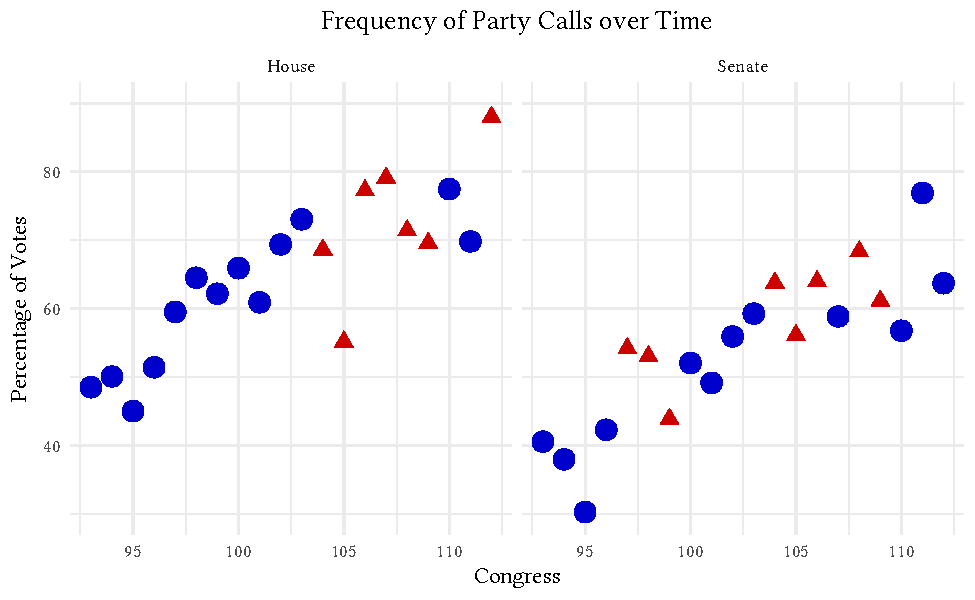
\includegraphics[width = \textwidth]{C:/Users/Ethan/Documents/GitHub/partycalls/plots/party_call_percent_both.pdf}
	\fnote{\textit{Note}: This figure shows the percentage of votes classified as party calls per Congress in each chamber. Blue circles denote Democrat majority Congresses while Red triangles denote Republican majority Congresses.}
\end{figure}

\noindent
It is possible that parties are calling more because increased ideological purity within them makes a party call more effective, or because they need members to rally more to get their agendas through. We believe that the underlying cause of this trend merits further investigation, but initially take it as evidence of much discussed increased partisanship and polarization in recent decades \cite{Lee:2009, Lee:2016, Theriault:2013, Smith:2014}. This trend holds regardless of which party is in the majority in the chamber.

Replications of the regression models of Minozzi \& Volden (shown in Tables 1 and 2) show the responsive extremists hypothesis to hold in our set of cases. This finding holds whether we consider all members together, or consider subsets by party or majority status. Below, in Figure 2, we show this to broadly hold when separate Congresses and majority party statuses are considered in each chamber.

We expected that reelection would make members less responsive to the call of the party as they work to pivot to their districts when approaching reelection. We find that for all models categories that the sign is in the expected direction and that for all, save Democrats, it achieves statistical significance. Further, we should expect that those retiring are no longer beholden to their constituents and thus would not have this draw on their attention when the party calls. We find across all models that retirees' responsiveness to party calls takes a positive coefficient and for all, save Democrats, it is statistically significant. 

We find that minority party women are substantially more responsive to party calls than their male counterparts in both chambers. Others have found that minority party women remain more focused on legislative agendas than their male counterparts \cite{Volden:2013}, and we take this finding as being in line with this account. While results for this are mixed, we find generally that increased same-party presidential vote share (an indicator of party strength in the district) increases responsiveness to party calls while increased personal vote share (an indicator of member popularity in the district) decreases responsiveness. However, this relationship does not present itself for Democrats. A number of factors complicate this relationship for Democrats, such as landslide presidential election losses and the presence of Southern Democrats early on who were more moderate than their copartisans.

\begin{table}[H]
	\begin{center}
		\singlespacing
		\small
		\caption{House Responsiveness to Party Calls}
		%\footnotesize
		\begin{tabular}{l c c c c c }
			\hline
			& All & Democrats & Republicans & Majority & Minority \\
			\hline
			Ideological Extremism & $7.766^{***}$  & $8.350^{***}$  & $5.873^{***}$  & $6.713^{***}$  & $8.655^{***}$  \\
			& $(0.130)$      & $(0.168)$      & $(0.207)$      & $(0.157)$      & $(0.201)$      \\
			Baseline Rate of Voting With Party              & $0.575^{***}$  & $0.636^{***}$  & $0.414^{***}$  & $0.522^{***}$  & $0.632^{***}$  \\
			& $(0.012)$      & $(0.015)$      & $(0.020)$      & $(0.015)$      & $(0.020)$      \\
			Vote Share            & $-0.007$       & $-0.058^{***}$ & $0.021$        & $-0.125^{***}$ & $-0.109^{***}$ \\
			& $(0.012)$      & $(0.013)$      & $(0.022)$      & $(0.015)$      & $(0.019)$      \\
			Pres. Vote Share      & $0.028^{**}$   & $0.099^{***}$  & $-0.098^{***}$ & $0.204^{***}$  & $0.185^{***}$  \\
			& $(0.010)$      & $(0.011)$      & $(0.020)$      & $(0.012)$      & $(0.018)$      \\
			Party Leader                 & $1.811^{***}$  & $1.972^{**}$   & $2.787^{***}$  & $2.627^{***}$  & $1.843^{**}$   \\
			& $(0.497)$      & $(0.599)$      & $(0.761)$      & $(0.647)$      & $(0.653)$      \\
			Committee Chair                  & $4.960^{***}$  & $2.552^{***}$  & $9.779^{***}$  & $1.964^{***}$  &                \\
			& $(0.456)$      & $(0.498)$      & $(0.803)$      & $(0.444)$      &                \\
			Power Committee                  & $2.756^{***}$  & $1.801^{***}$  & $2.931^{***}$  & $2.972^{***}$  & $1.135^{**}$   \\
			& $(0.235)$      & $(0.275)$      & $(0.374)$      & $(0.269)$      & $(0.361)$      \\
			Best Committee          & $-0.169^{***}$ & $-0.038^{*}$   & $-0.240^{***}$ & $-0.178^{***}$ & $-0.161^{***}$ \\
			& $(0.016)$      & $(0.019)$      & $(0.025)$      & $(0.019)$      & $(0.023)$      \\
			Female                 & $1.173^{***}$  & $0.615$        & $-0.078$       & $0.037$        & $2.228^{***}$  \\
			& $(0.322)$      & $(0.353)$      & $(0.574)$      & $(0.404)$      & $(0.442)$      \\
			African American                   & $1.835^{***}$  & $-0.470$       & $5.089$        & $-3.014^{***}$ & $3.402^{***}$  \\
			& $(0.429)$      & $(0.441)$      & $(2.972)$      & $(0.536)$      & $(0.610)$      \\
			Latino                 & $3.221^{***}$  & $1.711^{***}$  & $2.405^{*}$    & $2.453^{***}$  & $3.191^{***}$  \\
			& $(0.507)$      & $(0.514)$      & $(1.153)$      & $(0.626)$      & $(0.705)$      \\
			South                  & $-0.922^{***}$ & $-2.640^{***}$ & $3.610^{***}$  & $-2.180^{***}$ & $-0.667^{*}$   \\
			& $(0.205)$      & $(0.276)$      & $(0.329)$      & $(0.244)$      & $(0.313)$      \\
			Seniority              & $-0.053$       & $0.049$        & $-0.334^{***}$ & $0.011$        & $0.015$        \\
			& $(0.028)$      & $(0.031)$      & $(0.050)$      & $(0.034)$      & $(0.041)$      \\
			Freshman               & $0.834^{**}$   & $-0.058$       & $1.167^{*}$    & $0.346$        & $-0.456$       \\
			& $(0.297)$      & $(0.356)$      & $(0.464)$      & $(0.348)$      & $(0.446)$      \\
			Intercept            & $30.952^{***}$ & $21.282^{***}$ & $53.412^{***}$ & $30.032^{***}$ & $12.343^{***}$ \\
			& $(1.217)$      & $(1.495)$      & $(2.174)$      & $(1.390)$      & $(2.106)$      \\
			\hline
			R$^2$                  & 0.460          & 0.631          & 0.303          & 0.564          & 0.478          \\
			Adj. R$^2$             & 0.459          & 0.630          & 0.301          & 0.563          & 0.477          \\
			Num. obs.              & 8544           & 4746           & 3798           & 4898           & 3646           \\
			RMSE                   & 8.443          & 7.363          & 8.868          & 7.559          & 8.015          \\
			\hline
			\multicolumn{6}{l}{\scriptsize{$^{***}p<0.001$, $^{**}p<0.01$, $^*p<0.05$}}
		\end{tabular}
		\fnote{Results are produced by OLS regressions for all members for the entire period in the first column, with additional analyses for all Democrats and Republicans as well as all members of the Majority and Minority party in Congresses 93-112 in the House of Representatives. Details on the variables are provided in an appendix.}
	\end{center}
\end{table}

\begin{table}[H]
	\begin{center}
		\singlespacing
		\small
		\caption{Senate Responsiveness to Party Calls}
		%\footnotesize
		\begin{tabular}{l c c c c c }
			\hline
			& All & Democrats & Republicans & Majority & Minority \\
			\hline
			Ideological Extremism & $6.239^{***}$  & $3.136^{***}$ & $7.792^{***}$  & $4.708^{***}$  & $7.949^{***}$ \\
			& $(0.252)$      & $(0.409)$     & $(0.357)$      & $(0.315)$      & $(0.400)$     \\
			Baseline Rate of Voting with Party              & $0.737^{***}$  & $0.759^{***}$ & $0.742^{***}$  & $0.702^{***}$  & $0.702^{***}$ \\
			& $(0.021)$      & $(0.030)$     & $(0.031)$      & $(0.025)$      & $(0.035)$     \\
			Up For Reelection    & $-0.908^{*}$   & $-0.630$      & $-1.436^{**}$  & $-0.951^{*}$   & $-1.204^{*}$  \\
			& $(0.353)$      & $(0.426)$     & $(0.538)$      & $(0.411)$      & $(0.603)$     \\
			Retiree                & $2.103^{**}$   & $1.599$       & $2.290^{*}$    & $1.816^{*}$    & $2.575^{*}$   \\
			& $(0.693)$      & $(0.897)$     & $(0.997)$      & $(0.850)$      & $(1.110)$     \\
			Vote Share            & $0.029$        & $-0.053^{*}$  & $0.149^{***}$  & $-0.012$       & $0.076^{*}$   \\
			& $(0.018)$      & $(0.022)$     & $(0.028)$      & $(0.021)$      & $(0.030)$     \\
			Presidential Vote Share      & $0.097^{***}$  & $0.234^{***}$ & $-0.134^{***}$ & $0.182^{***}$  & $0.006$       \\
			& $(0.018)$      & $(0.024)$     & $(0.031)$      & $(0.020)$      & $(0.032)$     \\
			Party Leader                 & $1.604^{**}$   & $2.218^{**}$  & $0.910$        & $1.441^{*}$    & $1.940^{*}$   \\
			& $(0.539)$      & $(0.712)$     & $(0.776)$      & $(0.661)$      & $(0.899)$     \\
			Committee Chair                  & $2.105^{***}$  & $0.852$       & $3.626^{***}$  & $-0.017$       &               \\
			& $(0.452)$      & $(0.543)$     & $(0.700)$      & $(0.517)$      &               \\
			Power Committee       & $-0.684$       & $-0.855$      & $-0.325$       & $-0.052$       & $-1.468$      \\
			& $(0.620)$      & $(0.772)$     & $(0.924)$      & $(0.719)$      & $(1.064)$     \\
			Best Committee        & $0.163$        & $0.237$       & $0.008$        & $0.027$        & $0.373^{*}$   \\
			& $(0.101)$      & $(0.124)$     & $(0.154)$      & $(0.118)$      & $(0.174)$     \\
			Female                 & $2.041^{**}$   & $1.690^{*}$   & $0.451$        & $0.532$        & $4.256^{***}$ \\
			& $(0.638)$      & $(0.730)$     & $(1.132)$      & $(0.758)$      & $(1.113)$     \\
			African American                   & $-4.769$       & $-1.164$      & $-10.789^{*}$  & $1.531$        & $-5.519$      \\
			& $(2.486)$      & $(2.789)$     & $(4.278)$      & $(4.184)$      & $(3.219)$     \\
			Latino                 & $5.717^{**}$   & $1.814$       & $7.264^{**}$   & $4.781^{*}$    & $6.253$       \\
			& $(1.816)$      & $(2.198)$     & $(2.779)$      & $(1.878)$      & $(3.506)$     \\
			South                  & $0.613$        & $-1.690^{**}$ & $0.872$        & $0.054$        & $1.085$       \\
			& $(0.362)$      & $(0.557)$     & $(0.578)$      & $(0.427)$      & $(0.622)$     \\
			Seniority              & $0.002$        & $0.041$       & $-0.024$       & $0.077$        & $0.118$       \\
			& $(0.044)$      & $(0.052)$     & $(0.072)$      & $(0.060)$      & $(0.070)$     \\
			Freshman               & $0.859$        & $0.769$       & $0.358$        & $0.600$        & $0.996$       \\
			& $(0.566)$      & $(0.708)$     & $(0.842)$      & $(0.631)$      & $(1.032)$     \\
			Intercept            & $11.611^{***}$ & $9.447^{**}$  & $18.182^{***}$ & $16.365^{***}$ & $10.799^{**}$ \\
			& $(2.274)$      & $(2.906)$     & $(3.489)$      & $(2.644)$      & $(4.009)$     \\
			\hline
			R$^2$                  & 0.632          & 0.689         & 0.641          & 0.684          & 0.615         \\
			Adj. R$^2$             & 0.629          & 0.684         & 0.635          & 0.679          & 0.608         \\
			Num. obs.              & 1993           & 1042          & 951            & 1052           & 843           \\
			RMSE                   & 6.967          & 6.118         & 7.255          & 5.865          & 7.749         \\
			\hline
			\multicolumn{6}{l}{\scriptsize{$^{***}p<0.001$, $^{**}p<0.01$, $^*p<0.05$}}
		\end{tabular}
		\fnote{Results are produced by OLS regressions for all members for the entire period in the first column, with additional analyses for all Democrats and Republicans as well as all members of the Majority and Minority party in Congresses 93-112 in the Senate. Details on the variables are provided in an appendix.}
	\end{center}
\end{table}

Finally, we consider ideological extremism as a predictor for member behavior in each chamber broken down by Congress and majority party status. Across such divisions the responsive extremists hypothesis broadly holds. We note in the House that ideological extremism takes a positive coefficient for all but 4 cases and in the Senate for all but 2. Further, in the House, all positive coefficients are statistically significant and in the Senate 29 of the positive coefficients are statistically significant and 1 of the negative coefficients is. This provides added confidence in the aggregate results above.

\begin{figure}[H]
	\centering
	\caption{Ideology and Responsiveness to Party Calls, Congresses 93-112}
	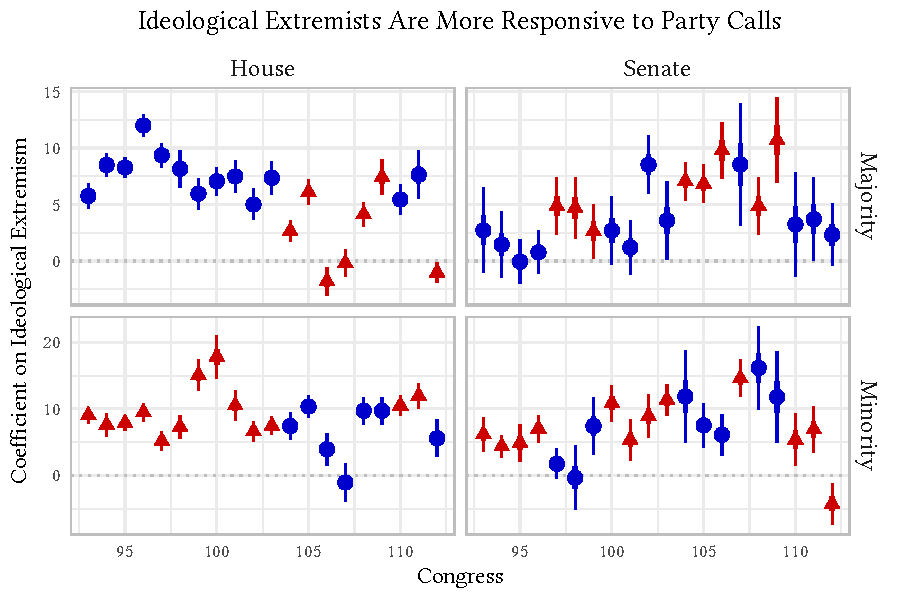
\includegraphics[width = 12cm]{C:/Users/Ethan/Documents/GitHub/partycalls/plots/both-chambers-figure2.pdf}
	\fnote{\textit{Note}: This coefficient plot is produced by the same formula shown in the House and Senate regression tables with results decomposed by individual Congresses for the Majority and Minority parties. Coefficients shown are for the effect of ideological extremism on party free votes in relation to party call votes. 50\% and 95\% confidence intervals are shown from the points.}
\end{figure} 

The models we have used in replicating \cite{Minozzi:2013} show correlation-based analyses of relationships between member traits and responsiveness to party calls. While they are not causal, they generate causal hypotheses. For instance, it now allows us to turn to considerations of whether being up for reelection causes a change in behavior on party call votes and only these votes. In doing so, we seek not only to further demonstrate the nature of this relationship, but also to demonstrate the usefulness of party call analysis more generally.

\subsection*{Reelection in the Senate}

In this section, we specifically consider the role of proximity to reelection in changing member roll call voting behavior on party free and party call votes. A member will have the preferences of their districts induced when they are up for reelection \cite{Levitt:1996}. So, we view it as likely that members up for reelection will use some party call votes to aid their personal - rather than the party - brand. Thus, we expect that members will be less responsive to the call of the party in a Congress they are up for reelection than they would at other points in their term.

To test this, we estimate models which rely on same-state Senator pairs when one of them is up for reelection at the end of the Congress. These pairings are ideal since same-state Senators are elected by the same districts, but not at the same time. This allows us to estimate a generalization of the difference-in-differences design. We use this to compare differences in responsiveness to party calls, baseline party voting rate, and the difference between these for members up for reelection. Differences between members from the same state should cancel each other out provided they both serve during the time the other is up for reelection, preventing us from getting spuriously significant findings.

\begin{figure}[H]
	\centering
	\caption{Voting Behavior Changes for Senators up for Reelection}
	
\includegraphics[width = 12cm]{C:/Users/Ethan/Documents/GitHub/partycalls/plots/senate_difference_estimates.pdf}
	\fnote{\textit{Note}: This coefficient plot is produced by a paired differences model which uses same-state Senators as a natural pairing. Estimates shown are the difference in responsiveness to party calls, baseline rate of voting with the party, and the difference in these differences. Bootstrapped 50\% and 95\% confidence intervals are shown.}
\end{figure}

We find member responsiveness to party calls declines, on average, about 1.5\% when they are up for reelection. However, their baseline rate of voting with the party is in line with what would be expected otherwise and the difference relative to baseline rate is about 1.25\%. During the period of analysis, 52\% of votes are classified as party calls and the average rate of responsiveness to party calls is 85\%. The average rate of voting with the party on non-party call votes is 82\%. Thus, while there is still an effect of the call of the party during a period of reelection, the induced preferences of the constituents reduces its impact.

Member voting behavior on other votes does not exhibit this relationship. Party call votes serve not only to establish brands for the party, but also for the members. Ignoring the call of the party at key times could allow Senators to stake out a more clear personal brand as they prepare for reelection. 

\subsection*{Conclusion}

In this paper, we tested if members respond to party calls in the Senate as they do in the House, using analyses based on those of Minozzi \& Volden (2013). In both chambers, recent times of increased ideological extremism and party division were associated with an increased incidence of party calls. Our results confirmed their responsive extremist hypothesis to hold in both chambers. 

We further showed reelection to reduce member response to party calls, but not their baseline rate of voting with the party. During this time, the preferences of the district are on the mind of legislators and thus we hypothesized - and found - that members up for reelection are less responsive to the party. This finding is in line with expectations of members working to consider voter preferences more highly as reelection becomes proximate. It expands on previous studies by highlighting the roll of party influenced votes in member decision-making when they are up for reelection. 

Having found this, we determine that party calls are an effective measure for the role of the party in roll call voting behavior. They allow the researcher to better decompose the often complementary roles of party and ideology in member vote decisions. Having shown this, we believe future work would do well to consider the separation of roll call votes by party calls and party free votes. 

\bibliographystyle{apsr}
\bibliography{senate}

\pagebreak

\section{Appendices}

\subsection{Appendix A: Detailing the New Sorting Algorithm}

As was done by Minozzi \& Volden (2013) we develop an algorithm to sort votes based on the degree to whether vote choice can be significantly predicted by party or caucus membership after ideology is accounted for. In this algorithm, member ideology in one iteration is calculated on the votes which were not party calls in the previous iteration since party is accounting for some of the weight in decision on the other set. Ideology for the first iteration is calculated on votes which have more than 65\% or less than 35\% of members of the chamber voting on the same side. The algorithm has a 15 iteration burn in period for each Congress. Once this has concluded, the algorithm continues either until the number of votes switched has hit a minimum and begun to climb or until there are fewer than 5 votes which switch between iterations. Once these conditions are met, it continues for 15 additional iterations, the last 5 of which are used to identify party calls and non calls. Any votes which switched between party calls and non party calls during the final 5 iterations are dropped from our analyses.

One of the key changes was the use of the \verb|binIRT()| R function from the \verb|emIRT|in order to calculate members' party free ideology, replacing \verb|ideal()| which was used by Minozzi \& Volden. The \verb|binIRT()| function was developed by Imai, Lo \& Olmsted in order to produce estimates analagous to those of \verb|ideal()| with reduced computational taxation. We find both of these aims to be met.

We find that the party call is not merely produced by a tradeoff of party and ideology explaining different votes; they are on the same side approximately two-thirds of the time in the House and three-fifths of the time in the Senate.

% latex table generated in R 3.3.2 by xtable 1.8-2 package
% Thu Feb 23 17:39:42 2017
\begin{table}[H]
	\centering
	\singlespacing
	\caption{House Sorting Algorithm Coefficient Signs}
	\begin{tabular}{rrr}
		\hline
		& ($-$) Ideal & (+) Ideal \\ 
		\hline
		(-) Party & 0.38 & 0.15 \\ 
		(+) Party & 0.17 & 0.30 \\ 
		\hline
	\end{tabular}
	\fnote{The party variable used in this analysis is an indicator for status as a Republican, and thus would be expected to correlate positively with ideal points.}
\end{table}

% latex table generated in R 3.3.2 by xtable 1.8-2 package
% Thu Feb 23 17:23:31 2017
\begin{table}[H]
	\centering
	\singlespacing
	\caption{Senate Sorting Algorithm Coefficient Signs}
	\begin{tabular}{rrr}
		\hline
		& ($-$) Ideal & (+) Ideal \\ 
		\hline
		($-$) Party & 0.33 & 0.16 \\ 
		(+) Party & 0.23 & 0.28 \\ 
		\hline
	\end{tabular}
	\fnote{The party variable used in this analysis is an indicator for status as a Republican, and thus would be expected to correlate positively with ideal points.}
\end{table}

We found that the lowered number of both members and bills in the Senate required a few changes to the vote sorting method, however. Since $p$-values will necessarily be lower with fewer observations, we had to change the threshold for party calls to $p <$ 0.05 (from $p <$ 0.01). Next, since the ideal point algorithm uses a logistic regression, problems arose in vote sorting when we also tried to use another to sort vote type with this in the Senate. Neither change leads the sorting in the House to differ for the most part. We find that the sorting of close and lopsided votes by this method to be in line with Minozzi \& Volden's findings.

% latex table generated in R 3.3.2 by xtable 1.8-2 package
% Mon Mar 20 13:02:44 2017
\begin{table}[H]
	\centering
	\singlespacing
	\caption{House Vote Coding for Close and Lopsided Votes} 
	\begin{tabular}{lrr}
		\hline
		& Party Call & Noncall \\ 
		\hline
		Lopsided & 4245 & 6123 \\ 
		Close & 9308 & 1090 \\ 
		\hline
	\end{tabular}
	\fnote{The threshold for a vote to be lopsided was 65\% of members (or conversely, 35\%) voting on the same side of a roll call vote.}
\end{table}

% latex table generated in R 3.3.2 by xtable 1.8-2 package
% Mon Mar 20 13:04:18 2017
\begin{table}[H]
	\centering
	\singlespacing
	\caption{Senate Vote Coding for Close and Lopsided Votes} 
	\begin{tabular}{lrr}
		\hline
		& Party Call & Noncall \\ 
		\hline
		Lopsided & 2063 & 4876 \\ 
		Close & 5233 & 1851 \\ 
		\hline
	\end{tabular}
	\fnote{The threshold for a vote to be lopsided was 65\% of members (or conversely, 35\%) voting on the same side of a roll call vote.}
\end{table}













\subsection{Appendix B: Methodology for Senate Reelection Section}

In order to better test the role of reelection we use same-state senators as a natural pairing. These results were shown in Figure 3 in the paper. The analyses we performed on these pairs were generalizations of the difference in differences design, in which the member not up for reelection had their rate of voting with the party on party calls and party free votes subtracted from that of the member who was up for reelection, as well as the difference between the response rate to party calls being subtracted from those of their same-state pairs. 

As a further test, not shown in the paper, we estimated the effect of reelection and other variables with a fixed effects model. This produces substantively similar effects to those reported in the main paper. This allows us to decompose results by party. In doing so, we find results largely in line with those reported in the paper. Democrats show the least changes as reelection approaches, but for all categories the effect of reelection on party call responsiveness is negative and statistically significant.

\begin{table}[H]
	\begin{center}
		\singlespacing
		\caption{Senate Fixed Effects Models}
		\begin{tabular}{l c c c c c }
			\hline
			& All & Democrats & Republicans & Majority & Minority \\
			\hline
			Ideological Extremism  & $2.36^{***}$  & $2.88^{***}$ & $4.00^{***}$  & $1.94^{**}$   & $4.11^{***}$ \\
			& $(0.48)$      & $(0.69)$     & $(0.75)$      & $(0.63)$      & $(0.88)$     \\
			Baseline Rate of Voting with Party               & $0.35^{***}$  & $0.37^{***}$ & $0.25^{***}$  & $0.38^{***}$  & $0.22^{**}$  \\
			& $(0.03)$      & $(0.05)$     & $(0.05)$      & $(0.05)$      & $(0.07)$     \\
			Up for Reelection     & $-1.01^{***}$ & $-0.55^{*}$  & $-1.55^{***}$ & $-1.03^{***}$ & $-0.91^{*}$  \\
			& $(0.25)$      & $(0.27)$     & $(0.34)$      & $(0.28)$      & $(0.36)$     \\
			Vote Share             & $-0.01$       & $0.03$       & $-0.05$       & $0.03$        & $-0.03$      \\
			& $(0.02)$      & $(0.02)$     & $(0.03)$      & $(0.03)$      & $(0.03)$     \\
			Pres. Vote Share       & $0.04$        & $0.27^{***}$ & $0.09$        & $0.32^{***}$  & $0.16^{**}$  \\
			& $(0.02)$      & $(0.04)$     & $(0.05)$      & $(0.06)$      & $(0.06)$     \\
			Freshman                & $1.31^{***}$  & $0.71$       & $0.98^{*}$    & $0.58$        & $0.64$       \\
			& $(0.37)$      & $(0.48)$     & $(0.46)$      & $(0.44)$      & $(0.76)$     \\
			Retiree                 & $0.52$        & $0.25$       & $0.88$        & $0.37$        & $0.60$       \\
			& $(0.63)$      & $(0.83)$     & $(0.83)$      & $(0.96)$      & $(0.85)$     \\
			Best Committee         & $0.18$        & $0.14$       & $0.11$        & $0.21$        & $0.32$       \\
			& $(0.10)$      & $(0.12)$     & $(0.16)$      & $(0.16)$      & $(0.17)$     \\
			Power Committee        & $-0.66$       & $-0.48$      & $-0.22$       & $-0.96$       & $-0.51$      \\
			& $(0.61)$      & $(0.70)$     & $(0.98)$      & $(0.88)$      & $(0.93)$     \\
			Party Leader                  & $1.27^{*}$    & $0.87$       & $1.46^{*}$    & $1.28$        & $1.12$       \\
			& $(0.51)$      & $(0.47)$     & $(0.62)$      & $(0.71)$      & $(0.74)$     \\
			Committee Chair                   & $2.93^{***}$  & $0.38$       & $0.65$        & $-0.36$       &              \\
			& $(0.48)$      & $(0.64)$     & $(0.71)$      & $(0.56)$      &              \\
			\hline
			Num. obs.               & 1993          & 1042         & 951           & 1100          & 893          \\
			R$^2$      & 0.87          & 0.89         & 0.91          & 0.91          & 0.93         \\
			Adj. R$^2$ & 0.85          & 0.87         & 0.88          & 0.88          & 0.90         \\
			\hline
			\multicolumn{6}{l}{\scriptsize{$^{***}p<0.001$, $^{**}p<0.01$, $^*p<0.05$}}
		\end{tabular}
	\end{center}
\end{table}

\section{Appendix C: Summary Statistics}

Here we give descriptions of report summary tables of the variables used in our paper. Members are grouped either as Democrats or Republicans, with independents being grouped with the party they caucus with in each chamber. The data are constructed with observations for members in each Congress they were present in. Values are according to member status in each Congress. Members who changed parties have multiple observations in the Congress which they did so in order to have observations for them in each. In each chamber, `Majority' is an indicator variable for if a members' party is in the majority during a Congress, which is used to divide results and summary statistics.\footnote{For the purposes of analyses, Congress 107 in the Senate was given Democrats as the majority party and Republicans as the minority party since this was the case for most - but not all - of the Congress. This decision does not meaningfully impact results.}

Variables were acquired from the Legislative Effectiveness Project (or constructed with those data) with a few exceptions. Roll call data are from Keith Krehbiel's corrected roll call datasets, which were used to identify and measure response to party calls and party free votes. Committee data for the Senate and Congresses 110-112 in the House are from Charles Stewart's Congressional data page, with committee value ranks coming from Grimmer \& Stewart (2013). Committee data from Congresses 93-109 in the House are taken from the replication data for Minozzi \& Volden (2013). House vote share data were provided to us by Gary Jacobson, Senate vote share data are from Dave Leip's U.S. Election Atlas. Senate retiree data were collected from the Congressional Bioguides. Gingrich Senators were identified based on Theriault (2013).

`Party Free Ideal Point' is a member's ideal point (calculated by \verb|binIRT()| from the \verb|emIRT()| R package) based on party free votes only. It is centered at 0 with a standard deviation of 1, with a requirement that Democrats' values are on average lower (further left) than Republicans'. `Ideological Extremism' is this value with sign reversed for Democrats such that higher numbers represent more extreme members for both parties. `Party Call Response Rate' is the percent of times that a member voted with a majority of their party on party call votes. `Baseline Rate of Voting with Party' is the percent of times a member votes with a majority of their party on non-party call votes. The theoretical minimum for this variable is 0 and the maximum is 100.

`Up for Reelection' is a Senate-specific variable, representing whether a member's election falls during a Congress. `Retiree' is an indicator variable for members who choose to leave office at or before the end of a Congress. `Vote Share' is calculated by the member's share of the vote relative to their nearest opponent.\footnote{In the House, we report above or below average centered at 0 since unchallenged runs were coded as missing, in order to avoid selecting values for these. This decision had no impact on results.}  `Pres. Vote Share' in each chamber is an indication of Democrat or Republican (depending on who the member caucused with) presidential candidate 2-party vote share in the previous election based on the previous presidential election.  `Party Leader' is an indicator for if a member is in one of the positions identified as the congressional leadership (other than committee positions) in the Almanac of American Politics for a particular Congress. `Committee Chair' is an indicator for if a member chairs a committee in Congress. `Power Committee' represents a member being on one of the top four committees.  `Best Committee' takes a value based on the best committee a member was on, with values ranging from 0 (not on a committee) to the number of committees in the chamber (on the best committee). `Female' is an indicator variable for female legislators. `African American' is an indicator for African American legislators. `Latino' is an indicator for Hispanic and Latino legislators. `South' is an indicator for if a member represents a state or district from 13-state south. `Seniority' is a count variable of the number of consecutive Congresses a member has served in. `Freshman' is an indicator variable for the first Congress of a member previously not in Congress. 



% Table created by stargazer v.5.2 by Marek Hlavac, Harvard University. E-mail: hlavac at fas.harvard.edu
% Date and time: Tue, May 16, 2017 - 11:58:48
\begin{table}[H] 
	\centering 
	\singlespacing
	\caption{Senate Summary Statistics, All} 
	\label{} 
	\begin{tabular}{@{\extracolsep{5pt}}lccccc} 
		\\[-1.8ex]\hline 
		\hline \\[-1.8ex] 
		Statistic & \multicolumn{1}{c}{N} & \multicolumn{1}{c}{Mean} & \multicolumn{1}{c}{St. Dev.} & \multicolumn{1}{c}{Min} & \multicolumn{1}{c}{Max} \\ 
		\hline \\[-1.8ex] 
		Party Free Ideal Point & 1,993 & 0.002 & 1.000 & $-$3.222 & 3.397 \\ 
		Ideological Extremism & 1,993 & 0.689 & 0.724 & $-$1.630 & 3.397 \\ 
		Party Call Response Rate & 1,993 & 85.491 & 11.438 & 8.777 & 100.000 \\ 
		Baseline Rate of Voting with Party & 1,993 & 82.035 & 8.164 & 45.106 & 100.000 \\ 
		Up for Reelection & 1,993 & 0.333 & 0.471 & 0 & 1 \\ 
		Retiree & 1,993 & 0.059 & 0.235 & 0 & 1 \\ 
		Vote Share & 1,993 & 0.612 & 0.099 & 0.500 & 1.000 \\ 
		Pres. Vote Share & 1,993 & 0.521 & 0.097 & 0.201 & 0.780 \\ 
		Party Leader & 1,993 & 0.099 & 0.299 & 0 & 1 \\ 
		Committee Chair & 1,993 & 0.183 & 0.386 & 0 & 1 \\ 
		Power Committee & 1,993 & 0.727 & 0.446 & 0 & 1 \\ 
		Best Committee & 1,993 & 12.277 & 2.740 & 0 & 15 \\ 
		Female & 1,993 & 0.067 & 0.250 & 0 & 1 \\ 
		African American & 1,993 & 0.004 & 0.063 & 0 & 1 \\ 
		Latino & 1,993 & 0.008 & 0.086 & 0 & 1 \\ 
		South & 1,993 & 0.260 & 0.439 & 0 & 1 \\ 
		Seniority & 1,993 & 6.254 & 4.618 & 1 & 26 \\ 
		Freshman & 1,993 & 0.114 & 0.318 & 0 & 1 \\ 
		
		\hline \\[-1.8ex] 
	\end{tabular} 
\end{table} 

% Table created by stargazer v.5.2 by Marek Hlavac, Harvard University. E-mail: hlavac at fas.harvard.edu
% Date and time: Tue, May 16, 2017 - 11:58:51
%\begin{table}[H] 
%	\centering 
%	\singlespacing
%	\caption{Senate Summary Statistics, Democrats} 
%	\label{} 
%	\begin{tabular}{@{\extracolsep{5pt}}lccccc} 
%		\\[-1.8ex]\hline 
%		\hline \\[-1.8ex] 
%		Statistic & \multicolumn{1}{c}{N} & \multicolumn{1}{c}{Mean} & \multicolumn{1}{c}{St. Dev.} & \multicolumn{1}{c}{Min} & \multicolumn{1}{c}{Max} \\ 
%		\hline \\[-1.8ex]  
%		Party Free Ideal Point & 1,042 & $-$0.657 & 0.657 & $-$3.222 & 1.630 \\ 
%		Ideological Extremism & 1,042 & 0.657 & 0.657 & $-$1.630 & 3.222 \\ 
%		Party Call Response Rate & 1,042 & 85.776 & 10.886 & 8.777 & 100.000 \\ 
%		Baseline Rate of Voting with Party & 1,042 & 83.760 & 7.862 & 45.106 & 100.000 \\
%		Up for Reelection & 1,042 & 0.334 & 0.472 & 0 & 1 \\ 
%		Retiree & 1,042 & 0.051 & 0.220 & 0 & 1 \\ 
%		Vote Share & 1,042 & 0.619 & 0.102 & 0.500 & 1.000 \\ 
%		Pres. Vote Share & 1,042 & 0.484 & 0.093 & 0.201 & 0.730 \\ 
%		Party Leader & 1,042 & 0.083 & 0.277 & 0 & 1 \\ 
%		Committee Chair & 1,042 & 0.208 & 0.406 & 0 & 1 \\ 
%		Power Committee & 1,042 & 0.729 & 0.445 & 0 & 1 \\ 
%		Best Committee & 1,042 & 12.257 & 2.780 & 0 & 15 \\ 
%		Female & 1,042 & 0.084 & 0.278 & 0 & 1 \\ 
%		African American & 1,042 & 0.005 & 0.069 & 0 & 1 \\ 
%		Latino & 1,042 & 0.008 & 0.087 & 0 & 1 \\ 
%		South & 1,042 & 0.236 & 0.425 & 0 & 1 \\ 
%		Seniority & 1,042 & 6.781 & 4.940 & 1 & 26 \\ 
%		Freshman & 1,042 & 0.105 & 0.306 & 0 & 1 \\  
%		\hline \\[-1.8ex] 
%	\end{tabular} 
%\end{table} 

% Table created by stargazer v.5.2 by Marek Hlavac, Harvard University. E-mail: hlavac at fas.harvard.edu
% Date and time: Tue, May 16, 2017 - 11:58:53
%\begin{table}[H] 
%	\centering 
%	\singlespacing
%	\caption{Senate Summary Statistics, Republicans} 
%	\label{} 
%	\begin{tabular}{@{\extracolsep{5pt}}lccccc} 
%		\\[-1.8ex]\hline 
%		\hline \\[-1.8ex] 
%		Statistic & \multicolumn{1}{c}{N} & \multicolumn{1}{c}{Mean} & \multicolumn{1}{c}{St. Dev.} & \multicolumn{1}{c}{Min} & \multicolumn{1}{c}{Max} \\ 
%		\hline \\[-1.8ex] 
%		Party Free Ideal Point & 951 & 0.725 & 0.789 & $-$1.595 & 3.397 \\ 
%		Party Call Response Rate & 951 & 85.180 & 12.011 & 33.232 & 100.000 \\ 
%		Baseline Rate of Voting with Party & 951 & 80.144 & 8.073 & 50.070 & 100.000 \\ 
%		Ideological Extremism & 951 & 0.725 & 0.789 & $-$1.595 & 3.397 \\ 		
%		Up for Reelection & 951 & 0.332 & 0.471 & 0 & 1 \\ 
%		Retiree & 951 & 0.067 & 0.251 & 0 & 1 \\ 
%		Vote Share & 951 & 0.605 & 0.094 & 0.500 & 1.000 \\ 
%		Pres. Vote Share & 951 & 0.562 & 0.085 & 0.310 & 0.780 \\ 
%		Leader & 951 & 0.117 & 0.321 & 0 & 1 \\ 
%		Committee Chair & 951 & 0.155 & 0.362 & 0 & 1 \\ 
%		Power Committee & 951 & 0.723 & 0.448 & 0 & 1 \\ 
%		Best Committee & 951 & 12.300 & 2.697 & 0 & 15 \\ 
%		Female & 951 & 0.048 & 0.215 & 0 & 1 \\ 
%		African American & 951 & 0.003 & 0.056 & 0 & 1 \\ 
%		Latino & 951 & 0.007 & 0.086 & 0 & 1 \\ 
%		South & 951 & 0.286 & 0.452 & 0 & 1 \\ 
%		Seniority & 951 & 5.677 & 4.163 & 1 & 24 \\ 
%		Freshman & 951 & 0.124 & 0.330 & 0 & 1 \\ 
%		\hline \\[-1.8ex] 
%	\end{tabular} 
%\end{table} 

% Table created by stargazer v.5.2 by Marek Hlavac, Harvard University. E-mail: hlavac at fas.harvard.edu
% Date and time: Tue, May 16, 2017 - 11:58:55
%\begin{table}[H] 
%	\centering 
%	\singlespacing
%	\caption{Senate Summary Statistics, Majority Party} 
%	\label{} 
%	\begin{tabular}{@{\extracolsep{5pt}}lccccc} 
%		\\[-1.8ex]\hline 
%		\hline \\[-1.8ex] 
%		Statistic & \multicolumn{1}{c}{N} & \multicolumn{1}{c}{Mean} & \multicolumn{1}{c}{St. Dev.} & \multicolumn{1}{c}{Min} & \multicolumn{1}{c}{Max} \\ 
%		\hline \\[-1.8ex] 
%		Party Free Ideal Point & 1,052 & $-$0.071 & 0.918 & $-$1.966 & 2.866 \\ 
%		Ideological Extremism & 1,052 & 0.614 & 0.687 & $-$1.630 & 2.866 \\ 
%		Party Call Response Rate & 1,052 & 86.934 & 10.350 & 37.020 & 100.000 \\ 
%		Baseeline Rate of Voting with Party & 1,052 & 83.089 & 8.216 & 45.106 & 100.000 \\ 		
%		Up for Reelection & 1,052 & 0.323 & 0.468 & 0 & 1 \\ 
%		Retiree & 1,052 & 0.051 & 0.221 & 0 & 1 \\ 
%		Vote Share & 1,052 & 0.614 & 0.100 & 0.500 & 1.000 \\ 
%		Pres. Vote Share & 1,052 & 0.506 & 0.101 & 0.201 & 0.780 \\ 
%		Party Leader & 1,052 & 0.096 & 0.295 & 0 & 1 \\ 
%		Committee Chair & 1,052 & 0.329 & 0.470 & 0 & 1 \\ 
%		Power Committee & 1,052 & 0.721 & 0.449 & 0 & 1 \\ 
%		Best Committee & 1,052 & 12.270 & 2.755 & 0 & 15 \\ 
%		Female & 1,052 & 0.065 & 0.246 & 0 & 1 \\ 
%		African American & 1,052 & 0.002 & 0.044 & 0 & 1 \\ 
%		Latino & 1,052 & 0.010 & 0.097 & 0 & 1 \\ 
%		South & 1,052 & 0.267 & 0.443 & 0 & 1 \\ 
%		Seniority & 1,052 & 6.089 & 4.618 & 1 & 26 \\ 
%		Freshman & 1,052 & 0.129 & 0.336 & 0 & 1 \\ 
%		
%		\hline \\[-1.8ex] 
%	\end{tabular} 
%\end{table} 


% Table created by stargazer v.5.2 by Marek Hlavac, Harvard University. E-mail: hlavac at fas.harvard.edu
% Date and time: Tue, May 16, 2017 - 11:58:57
%\begin{table}[H] 
%	\centering 
%	\singlespacing
%	\caption{Senate Summary Statistics, Minority Party } 
%	\label{} 
%	\begin{tabular}{@{\extracolsep{5pt}}lccccc} 
%		\\[-1.8ex]\hline 
%		\hline \\[-1.8ex] 
%		Statistic & \multicolumn{1}{c}{N} & \multicolumn{1}{c}{Mean} & \multicolumn{1}{c}{St. Dev.} & \multicolumn{1}{c}{Min} & \multicolumn{1}{c}{Max} \\ 
%		\hline \\[-1.8ex] 
%		
%		Party Free Ideal Point & 843 & 0.091 & 1.086 & $-$3.222 & 3.397 \\ 
%		Ideological Extremism & 843 & 0.767 & 0.773 & $-$1.269 & 3.397 \\ 		
%		Party Call Response Rate & 843 & 83.138 & 12.372 & 8.777 & 100.000 \\ 
%		Baseline Rate of Voting with Party & 843 & 80.354 & 8.068 & 50.070 & 100.000 \\ 		
%		Up for Reelection & 843 & 0.345 & 0.476 & 0 & 1 \\ 
%		Retiree & 843 & 0.070 & 0.255 & 0 & 1 \\ 
%		Vote Share & 843 & 0.611 & 0.098 & 0.500 & 1.000 \\ 
%		Pres. Vote Share & 843 & 0.538 & 0.091 & 0.284 & 0.754 \\ 
%		Party Leader & 843 & 0.102 & 0.303 & 0 & 1 \\ 
%		Committee Chair & 843 & 0.000 & 0.000 & 0 & 0 \\ 
%		Power Committee & 843 & 0.733 & 0.443 & 0 & 1 \\ 
%		Best Committee & 843 & 12.284 & 2.711 & 0 & 15 \\ 
%		Female & 843 & 0.064 & 0.245 & 0 & 1 \\ 
%		African American & 843 & 0.007 & 0.084 & 0 & 1 \\ 
%		Latino & 843 & 0.006 & 0.077 & 0 & 1 \\ 
%		South & 843 & 0.250 & 0.433 & 0 & 1 \\ 
%		Seniority & 843 & 6.409 & 4.545 & 1 & 24 \\ 
%		Freshman & 843 & 0.096 & 0.295 & 0 & 1 \\ 
%		\hline \\[-1.8ex] 
%	\end{tabular} 
%\end{table} 

% Table created by stargazer v.5.2 by Marek Hlavac, Harvard University. E-mail: hlavac at fas.harvard.edu
% Date and time: Tue, May 16, 2017 - 12:20:30
\begin{table}[H] 
	\centering 
	\singlespacing
	\caption{House Summary Statistics, All} 
	\label{} 
	\begin{tabular}{@{\extracolsep{5pt}}lccccc} 
		\\[-1.8ex]\hline 
		\hline \\[-1.8ex] 
		Statistic & \multicolumn{1}{c}{N} & \multicolumn{1}{c}{Mean} & \multicolumn{1}{c}{St. Dev.} & \multicolumn{1}{c}{Min} & \multicolumn{1}{c}{Max} \\ 
		\hline \\[-1.8ex]  
		Democrat & 8,544 & 0.555 & 0.497 & 0 & 1 \\ 
		Majority & 8,544 & 0.573 & 0.495 & 0 & 1 \\ 
		Female & 8,544 & 0.094 & 0.292 & 0 & 1 \\ 
		African American & 8,544 & 0.063 & 0.244 & 0 & 1 \\ 
		Latino & 8,544 & 0.035 & 0.183 & 0 & 1 \\ 
		Committee Chair & 8,544 & 0.051 & 0.219 & 0 & 1 \\ \ 
		Power Committee & 8,544 & 0.255 & 0.436 & 0 & 1 \\ 
		Seniority & 8,544 & 5.331 & 4.054 & 1 & 29 \\ 
		South & 8,544 & 0.296 & 0.456 & 0 & 1 \\ 
		Freshman & 8,544 & 0.156 & 0.363 & 0 & 1 \\ 
		Party Leader & 8,544 & 0.036 & 0.187 & 0 & 1 \\  
		Pres. Vote Share & 8,544 & 56.578 & 12.357 & 16.310 & 96.060 \\ 
		Vote Share vs. Mean Vote Share & 8,544 & $-$0.000 & 9.150 & $-$15.727 & 31.353 \\ 
		Best Committee & 8,544 & 13.822 & 6.376 & 0 & 22 \\ 
		Party Free Ideal Point & 8,544 & $-$0.004 & 1.003 & $-$4.076 & 9.347 \\ 
		Ideological Extremism & 8,544 & 0.603 & 0.802 & $-$4.317 & 9.347 \\ 
		Party Call Response Rate & 8,544 & 85.800 & 11.478 & 8.021 & 100.000 \\ 
		Baseline Rate of Voting With Party & 8,544 & 86.955 & 7.507 & 0.000 & 100.000 \\ 
		\hline \\[-1.8ex] 
	\end{tabular} 
\end{table} 

% Table created by stargazer v.5.2 by Marek Hlavac, Harvard University. E-mail: hlavac at fas.harvard.edu
% Date and time: Tue, May 16, 2017 - 12:20:33
%\begin{table}[H] 
%	\centering 
%	\singlespacing
%	\caption{House Summary Statistics, Democrats} 
%	\label{} 
%	\begin{tabular}{@{\extracolsep{5pt}}lccccc} 
%		\\[-1.8ex]\hline 
%		\hline \\[-1.8ex] 
%		Statistic & \multicolumn{1}{c}{N} & \multicolumn{1}{c}{Mean} & \multicolumn{1}{c}{St. Dev.} & \multicolumn{1}{c}{Min} & \multicolumn{1}{c}{Max} \\ 
%		\hline \\[-1.8ex]  
%		Party Free Ideal Point & 4,746 & $-$0.546 & 0.809 & $-$4.076 & 4.317 \\ 
%		Party Call Response Rate & 4,746 & 86.290 & 12.110 & 8.021 & 100.000 \\ 
%		Baseline Rate of Voting with Party & 4,746 & 86.996 & 7.214 & 0.000 & 100.000 \\ 
%		Ideological Extremism & 4,746 & 0.546 & 0.809 & $-$4.317 & 4.076 \\ 
%		Vote Share vs. Mean Vote Share & 4,746 & 1.319 & 9.905 & $-$15.727 & 31.353 \\
%		Pres. Vote Share & 4,746 & 54.871 & 14.495 & 16.310 & 96.060 \\ 
%		Party Leader & 4,746 & 0.034 & 0.182 & 0 & 1 \\ 
%		Committee Chair & 4,746 & 0.062 & 0.240 & 0 & 1 \\
%		Power Committee & 4,746 & 0.257 & 0.437 & 0 & 1 \\
%		Best Committee & 4,746 & 13.832 & 6.398 & 0 & 22 \\
%		Female & 4,746 & 0.114 & 0.317 & 0 & 1 \\ 
%		African American & 4,746 & 0.112 & 0.316 & 0 & 1 \\ 
%		Latino & 4,746 & 0.050 & 0.217 & 0 & 1 \\ 
%		South & 4,746 & 0.289 & 0.453 & 0 & 1 \\ 		 
%		Seniority & 4,746 & 5.752 & 4.376 & 1 & 29 \\ 
%		Freshman & 4,746 & 0.140 & 0.347 & 0 & 1 \\ 
%		\hline \\[-1.8ex] 
%	\end{tabular} 
%\end{table} 

% Table created by stargazer v.5.2 by Marek Hlavac, Harvard University. E-mail: hlavac at fas.harvard.edu
% Date and time: Tue, May 16, 2017 - 12:20:35
%\begin{table}[H] 
%	\centering 
%	\singlespacing
%	\caption{House Summary Stats, Republicans} 
%	\label{} 
%	\begin{tabular}{@{\extracolsep{5pt}}lccccc} 
%		\\[-1.8ex]\hline 
%		\hline \\[-1.8ex] 
%		Statistic & \multicolumn{1}{c}{N} & \multicolumn{1}{c}{Mean} & \multicolumn{1}{c}{St. Dev.} & \multicolumn{1}{c}{Min} & \multicolumn{1}{c}{Max} \\ 
%		\hline \\[-1.8ex] 
%		Party Free Ideal Point & 3,798 & 0.674 & 0.786 & $-$2.473 & 9.347 \\ 
%		Ideological Extremism & 3,798 & 0.674 & 0.786 & $-$2.473 & 9.347 \\ 	
%		Party Call Response Rate & 3,798 & 85.186 & 10.605 & 31.276 & 100.000 \\ 
%		Baseline Rate of Voting with Party & 3,798 & 86.904 & 7.858 & 28.302 & 100.000 \\
%		Vote Share vs. Mean Vote Share & 3,798 & $-$1.648 & 7.801 & $-$15.707 & 25.673 \\
%		Pres. Vote Share & 3,798 & 58.710 & 8.534 & 23.470 & 86.830 \\
%		Party Leader & 3,798 & 0.039 & 0.193 & 0 & 1 \\ 
%		Committee Chair & 3,798 & 0.037 & 0.189 & 0 & 1 \\ 
%		Power Committee & 3,798 & 0.251 & 0.434 & 0 & 1 \\ 
%		Best Committee & 3,798 & 13.810 & 6.349 & 0 & 22 \\ 
%		Female & 3,798 & 0.069 & 0.254 & 0 & 1 \\ 
%		African American & 3,798 & 0.002 & 0.049 & 0 & 1 \\ 
%		Latino & 3,798 & 0.016 & 0.126 & 0 & 1 \\ 
%		South & 3,798 & 0.304 & 0.460 & 0 & 1 \\
%		Seniority & 3,798 & 4.805 & 3.543 & 1 & 21 \\  
%		Freshman & 3,798 & 0.176 & 0.381 & 0 & 1 \\		 
%		\hline \\[-1.8ex] 
%	\end{tabular} 
%\end{table} 

% Table created by stargazer v.5.2 by Marek Hlavac, Harvard University. E-mail: hlavac at fas.harvard.edu
% Date and time: Tue, May 16, 2017 - 12:20:37
%\begin{table}[H] 
%	\centering 
%	\singlespacing
%	\caption{House Summary Statistics, Majority Party} 
%	\label{} 
%	\begin{tabular}{@{\extracolsep{5pt}}lccccc} 
%		\\[-1.8ex]\hline 
%		\hline \\[-1.8ex] 
%		Statistic & \multicolumn{1}{c}{N} & \multicolumn{1}{c}{Mean} & \multicolumn{1}{c}{St. Dev.} & \%multicolumn{1}{c}{Min} & \multicolumn{1}{c}{Max} \\ 
%		\hline \\[-1.8ex]  
%		Party Free Ideal Point & 4,898 & $-$0.153 & 0.957 & $-$4.076 & 9.347 \\  
%		Ideological Extremism & 4,898 & 0.526 & 0.814 & $-$4.317 & 9.347 \\ 
%		Party Call Response Rate & 4,898 & 87.607 & 11.437 & 8.021 & 100.000 \\ 
%		Baseline Rate of Voting with Party & 4,898 & 87.071 & 7.584 & 0.000 & 100.000 \\
%	 	Vote Share vs. Mean Vote Share & 4,898 & 0.518 & 9.087 & $-$15.727 & 31.243 \\ 
%	 	Pres. Vote Share & 4,898 & 52.854 & 12.457 & 16.310 & 96.060 \\
%	 	Party Leader & 4,898 & 0.030 & 0.170 & 0 & 1 \\ 
%	 	Committee Chair & 4,898 & 0.088 & 0.284 & 0 & 1 \\ 
%	 	Power Committee & 4,898 & 0.275 & 0.447 & 0 & 1 \\ 
%	 	Best Committee & 4,898 & 14.133 & 6.333 & 0 & 22 \\ 
%		Female & 4,898 & 0.082 & 0.274 & 0 & 1 \\ 
%		African American & 4,898 & 0.060 & 0.238 & 0 & 1 \\ 
%		Latino & 4,898 & 0.032 & 0.176 & 0 & 1 \\  
%		South & 4,898 & 0.323 & 0.468 & 0 & 1 \\
%		Seniority & 4,898 & 5.390 & 4.207 & 1 & 28 \\   
%		Freshman & 4,898 & 0.166 & 0.372 & 0 & 1 \\ 
%		\hline \\[-1.8ex] 
%	\end{tabular} 
%\end{table} 

% Table created by stargazer v.5.2 by Marek Hlavac, Harvard University. E-mail: hlavac at fas.harvard.edu
% Date and time: Tue, May 16, 2017 - 12:20:39
%\begin{table}[H] 
%	\centering 
%	\singlespacing
%	\caption{House Summary Statistics, Minority Party} 
%	\label{} 
%	\begin{tabular}{@{\extracolsep{5pt}}lccccc} 
%		\\[-1.8ex]\hline 
%		\hline \\[-1.8ex] 
%		Statistic & \multicolumn{1}{c}{N} & \multicolumn{1}{c}{Mean} & \multicolumn{1}{c}{St. Dev.} & \multicolumn{1}{c}{Min} & \multicolumn{1}{c}{Max} \\ 
%		\hline \\[-1.8ex] 
%		Party Free Ideal Point & 3,646 & 0.197 & 1.028 & $-$3.524 & 4.084 \\ 
%		Ideological Extremism & 3,646 & 0.706 & 0.773 & $-$1.756 & 4.084 \\ 
%		Party Call Response Rate & 3,646 & 83.371 & 11.079 & 20.077 & 100.000 \\ 
%		Baseline Rate of Voting with Party & 3,646 & 86.800 & 7.400 & 38.889 & 100.000 \\ 
%		Vote Share vs. Mean Vote Share & 3,646 & $-$0.696 & 9.188 & $-$15.717 & 31.353 \\
%		Pres. Vote Share & 3,646 & 61.580 & 10.284 & 23.470 & 96.050 \\ 
%		Party Leader & 3,646 & 0.045 & 0.207 & 0 & 1 \\ 
%		Committee Chair & 3,646 & 0.000 & 0.000 & 0 & 0 \\ 
%		Power Committee & 3,646 & 0.227 & 0.419 & 0 & 1 \\ 
%		Best Committee & 3,646 & 13.404 & 6.410 & 0 & 22 \\ 
%		Female & 3,646 & 0.110 & 0.313 & 0 & 1 \\ 
%		African American & 3,646 & 0.067 & 0.251 & 0 & 1 \\ 
%		Latino & 3,646 & 0.039 & 0.193 & 0 & 1 \\ 
%		South & 3,646 & 0.259 & 0.438 & 0 & 1 \\		
%		Seniority & 3,646 & 5.251 & 3.838 & 1 & 29 \\  
%		Freshman & 3,646 & 0.142 & 0.349 & 0 & 1 \\ 		 
%		\hline \\[-1.8ex] 
%	\end{tabular} 
%\end{table} 




















































\end{document}